% Write the report here. You can use the nested imports via 'subimport', see the following link:
% https://www.overleaf.com/learn/latex/Management_in_a_large_project#Using_the_import_package
% You also can see an example at line n.16.

\section{Основные понятия}
Определим несколько понятий, которые понадобятся нам в дальнейшем.
\begin{definition}
    \textbf{Бид} (bid) --- это самая высокая цена, которую покупатель готов заплатить за актив. 
    Далее, бид в момент времени $t$ будет обозначаться $B_t$.
    \textbf{Аск} (ask) --- это самая низкая цена, за которую продавец готов предоставить актив. 
    Далее, аск в момент времени $t$ будет обозначаться $B_t$.
    \textbf{Бид-аск спрэд} (bid–ask spread) $s$: $s = A_t - B_t$.
    \textbf{Мид} (mid-quote price): $V_{t} = \frac{A_{t} + B_{t}}{2}$.
\end{definition}
Начнем с рассмотрения структуры лимитной книги заявок (Limit Order Book -- LOB). 
В рамках этой парадигмы организации биржевых торгов, у каждого участника есть две возможности:
\begin{itemize}
    \item выразить желание купить или продать определённое количество единиц актива по определенной цене. 
    В этом случае, биржа запомнит пару цена--количество. Множество этих пар составляет 
    лимитную книгу заявок. На рисунке \ref{LOBpic} изображено традиционное представление лимитной
    книги заявок.
    \item выразить желание купить или продать определённое количество единиц актива немедленно. 
    В этом случае он немедленно получит запрошенное количество акций (если на бирже есть необходимое количество)
    по лучшей возможной цене: к примеру, в случае покупки, если на верхнем ценовом уровне не будет достаточного
    количества единиц актива для удовлетворения заявки, то будут взяты активы из следующего ценового уровня.
    Таким образом, не гарантируется, что итоговая цена одной единицы актива будет совпадать с аском.
    
\end{itemize}

\begin{figure}
    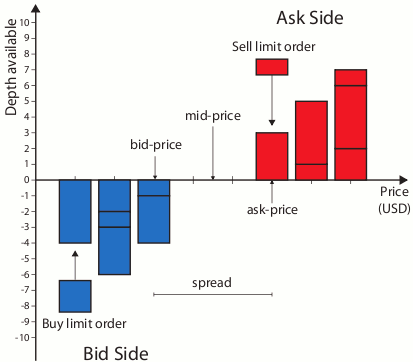
\includegraphics[scale=0.8]{fig/Graphical-representation-of-the-Limit-Order-Book.png}
    \caption{Графическое представление лимитной книги заявок}
    \label{LOBpic}
\end{figure}



Таким образом, если опустить некоторые подробности, существует два вида заявок:
\begin{definition}
    \textbf{Лимитная заявка (ордер)}(limit order) представляет собой распоряжение на покупку или продажу ценной бумаги по определенной цене или выше. 
    Этот тип заявки гарантирует цену исполнения, но не гарантирует само исполнение.
\end{definition}
\begin{definition}
    \textbf{Рыночная заявка (ордер)} (market order) представляет собой распоряжение на немедленную покупку или продажу ценной бумаги. 
    Этот тип заявки гарантирует, что она будет исполнена, но не гарантирует цену исполнения.
\end{definition}

% \begin{figure}
%     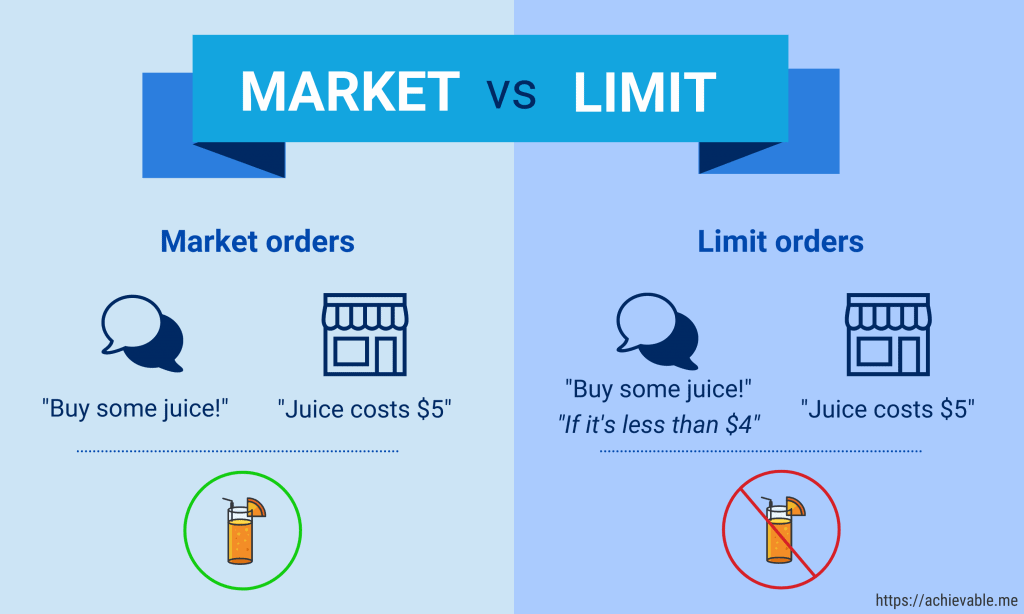
\includegraphics[scale=0.4]{fig/market-vs-limit-1024x614.png}
%     \caption{The difference between market order and limit order}
%     \label{fig:mvslim}
% \end{figure}

Теперь ясно, что если мы хотим продать или купить актив в количестве, достаточно большом, чтобы он мог оказать существенное
влияние на рынок, мы не должны делать это одной заявкой: это было бы очень дорого, поскольку крупный ордер
удалил бы все верхние уровни в лимитной книге заявок. Поэтому на практике все крупные заявки разбиваются на большое количество мелких.
Например, можно просто разделить ордер на N равных частей и продавать их через равные промежутки времени (это называется TWAP).
Но есть ли лучшее решение?


\section{Подход Обижаевой и Ванга к формализации проблемы}
В попытке найти лучшее решение, мы рассматриваем модель Обижаевой--Ванга,
в терминах которой задача имеет следующий вид: \par
\begin{align*} \label{oEproblem}
    J_0 &= \min _{\{x_0 \cdots x_N \}} E_0 \left[ \sum _{n=0}^N [A_{t_n} + x_n /(2q)] x_n\right],  \\
    A_{t_n} &= F_{t_n} + \lambda (X_0 - X_{t_n}) + s/2 + \sum _{i=0}^{n-1} x_i \kappa e^{- \rho \tau (n - i)},
 \end{align*}
 
где
\begin{itemize}
 \item трейдер должен купить $\mathbf{X_0}$ единиц актива за фиксированный период времени $[0,T]$;
 \item $x_{t_n}$ размер оредра в момент времени $t_n = \tau n$ (здесь, $\tau = T / N$); 
 \item $X_{t_n} := X_0 - \sum _{t_k < t_n} x_{t_k}$;
 \item $B_{t_n}$ и $A_{t_n}$ --- бид и аск в момент времени $t_n$; 
 \item $V_{t_n} = \frac{A_{t_n} + B_{t_n}}{2}$ --- мид; 
 \item $s$ --- бид-аск спрэд;
 \item $F_t$ --- фундаментальная (справедливая) цена актива;
 \item $q(P)$ распределение лимитной книги заявок $P$ (по ценам $[a, b]$ доступно $\int_a^b q(p) dP$ единиц актива);
 % \item $q$, $\lambda$ and $\rho$ is a LOB density, the permanent price impact and the resiliency.
 \item параметр $\lambda$ --- постоянный маркет импакт (справдливая цена $V_t$ в результате исполнения ордера объема $x$ меняется по закону: $V_{t+} = V_t + \lambda x$);
  \item $\kappa = \frac{1}{q} - \lambda $;
 \item параметр $\rho$ --- упргуость стакана (resiliency).
\end{itemize}

Данная задача была решена в статье \cite{obizhaeva2013optimal}:
\begin{theorem}
    Решение проблемы оптимального исполнения:
    \begin{multline*}
        x_n = - \frac{1}{2} \delta_{n + 1} [D_{t_n} (1 - \beta_{n + 1} e^{ - \rho \tau} + 2 \kappa \gamma_{n+1} e^{ - 2 \rho \tau}) 
         - X_{t_n} (\lambda + 2 \alpha_{n+1} - \beta_{n+1}\kappa e^{ - \rho \tau}) ], 
    \end{multline*}
    где $x_N = X_N$ и $D_t = A_t - V_t - s/2$. Ожидаемая цена будущих сделок в рамках
    стратегии оптимального исполнения меняется по закону
    \begin{equation*}
        J_{t_n} = (F_{t_n} + s/2) X_{t_n} + \lambda X_0 X_{t_n} + \alpha_n X_{t_n} ^2 + \beta_{n} D_{t_n} X_{t_n} + \gamma_n D_{t_n}^2, 
    \end{equation*}
    где коэффициенты $\alpha_{n+1}$, $\beta_{n+1}$, $\gamma_{n+1}$ и $\delta_{n+1}$ определяются рекурснивно по формулам:
    \begin{equation*}
        \alpha_{n} = \alpha_{n+1} - \frac{1}{4} \delta _{n+1} (\lambda + 2 \alpha_{n+1} - \beta_{n+1} \kappa e^{- \rho \tau})^2, 
    \end{equation*}
    \begin{multline*}
        \beta_{n} =  \beta_{n+1} e^{- \rho \tau} + \frac{1}{2} \delta _{n+1} (1 - \beta_{n+1} e^{- \rho \tau} 
         + 2 \kappa \gamma_{n+1} e^{- 2 \rho \tau}) (\lambda + 2 \alpha_{n+1} - \beta_{n+1} \kappa e^{-\rho \tau}), 
    \end{multline*}
    \begin{equation*}
         \gamma_n =   \gamma_{n+1} e^{- 2 \rho \tau} - \frac{1}{4} \delta _{n+1} (1 - \beta _{n+1} e^{- \rho \tau} 
    + 2 \gamma _{n+1} \kappa e^{- 2 \rho \tau})^2, 
    \end{equation*}
    где $\delta_{n+1} = [1/(2q) + \alpha_{n+1} - \beta_{n+1} \kappa e^{-\rho \tau} + \gamma _{n+1} \kappa ^2 e^{- 2 \rho \tau}]^{-1}$ и начальные условия
    \begin{equation*}
        \alpha_{N} = 1/(2q) - \lambda, \;\;\;\;\;\;\; \beta_N = 1, \;\;\;\;\;\;\; \gamma_N = 0.
    \end{equation*}
\end{theorem}

В нашем исследовании мы будем рассматривать предел этого решения.

\begin{theorem}
    Пии $N \rightarrow \infty$, стратегия оптимального исполнения принимает вид:
    \begin{align*}
        & \lim _{N \rightarrow \infty} x_0 = x_{t = 0} = \frac{X_0}{\rho T + 2}, \\
        & \lim _{N \rightarrow \infty} x_n / (T/N) = \dot X _t = \frac{\rho X_0}{\rho T + 2}, \;\;\;\;\;\; t \in (0, T), \\
        & \lim _{N \rightarrow \infty} x_0 = x_{t = 0} = \lim _{N \rightarrow \infty} x_n / (T/N) = x_{t=T}=  \frac{X_0}{\rho T + 2}.  %\\
    \end{align*}
    где $x_0$ первая сделка за отведенный период, $x_N$ --- последняя, и $\dot X _t$ скорость трейдинга между ними.
\end{theorem}

Таким образом, мы имеем явную формулу для стратегии оптимального исполнения. Но нам необходимо каким-либо образом найти
параметры $\rho, \kappa$ и $\lambda$ для того, чтобы применить её на практике. 

\section{Как подобрать параметры?}

Мы предлагаем наш метод для их нахождения: 
\begin{theorem}
    Для упрощения записей введём обозначения:
    \[
    A_k := A_{t_k}, \; \; \; \; 
    x_{k}:= x_{t_k}, \; \; \; \; 
    \Delta t_{k+1} := t_{k+1} - t_k, \; \; \; \;   
    \Delta A_{k+1} := A_{k+1} - A_k. 
    \]
        Если $\rho \Delta t << 1$, то в регрессии                                                                                                                                                                                                                                                                                                                                                                                     
        \begin{equation*}
            \frac{\Delta A_{k+2}}{\Delta t_{k+2}} - \frac{\Delta A_{k+1}}{\Delta t_{k+1}} 
        = -\rho \Delta A_k + \rho (\lambda + \kappa) x_{t_k} - \rho \kappa x_{t_{k+1}} 
        + (\lambda + \kappa) \left(\frac{x_{t_{k+1}}}{\Delta t_{k+1}} - \frac{x_{t_k}}{\Delta t_{k}}\right),
        \end{equation*}
        где $x_{k}$ и $A_{k}$ глубина ордера и аск в момент времени $t_k$, соответственно, \\

        коэффициенты $\rho, \kappa$ и $\lambda$ примерно те же, что в модели Обижаевой--Ванга, описывающей рынок,
        характеризуемый временными рядами: $A_k, \Delta t _k, x_k$.



\end{theorem}

Вся требуемая информация может быть получена из l3 данных: 
\begin{itemize}
    \item $\Delta A_{k}$ изменение аска в следствие исполнения заявки размера $x_k$ в момент времени $t_k$.
    \item $\Delta t_{k}$ время между $k$ и $k + 1$ заявками.
\end{itemize}

Другая идея связана с рассмотрением уравнения, задающего динамику изменения аска после исполнения крупного ордера (глубины $x_1$):
\begin{equation*}
        A_t = \overline p _t + \frac{s}{2} + x_1 \kappa e^{- \rho t}.
\end{equation*}
Она выглядит хорошо, но сопряжена с существенными численными сложностями: мы протестировали несколько подходов, связанных
с этой идеей, но нам не удалось извлечь адекватные параметры.



\section{Данные}
\subsection{Источники и обработка}
Мы работали с ордерлогами (\href{https://fs.moex.com/f/3198/specifikacija-formata-dannyh.pdf}{спецификация}). Было написано несколько 
\href{https://github.com/VsevolodZaostrovsky/OWModel/tree/main/New%20data/data%20preparing}{программ},
которые, в совокупности, распаршивали исходные записи в таблицу из четвёрок (время, аск до исполнения ордера, аск после исполнения ордера, глубина ордера). 
Следует обратить внимание на то, что заявки, поглощающие несколько уровней, представляются в данных в виде последовательности заявок, поэтому 
перед началом обработки их следует объединить: объем ордера есть сумма объемов, аск до исполнения --- аск до исполнения первого ордера,
аск после исполнения --- аск после исполнения последнего ордера. Фрагмент таблицы изображен на рисунке \ref{datacsv}.
\begin{figure}
    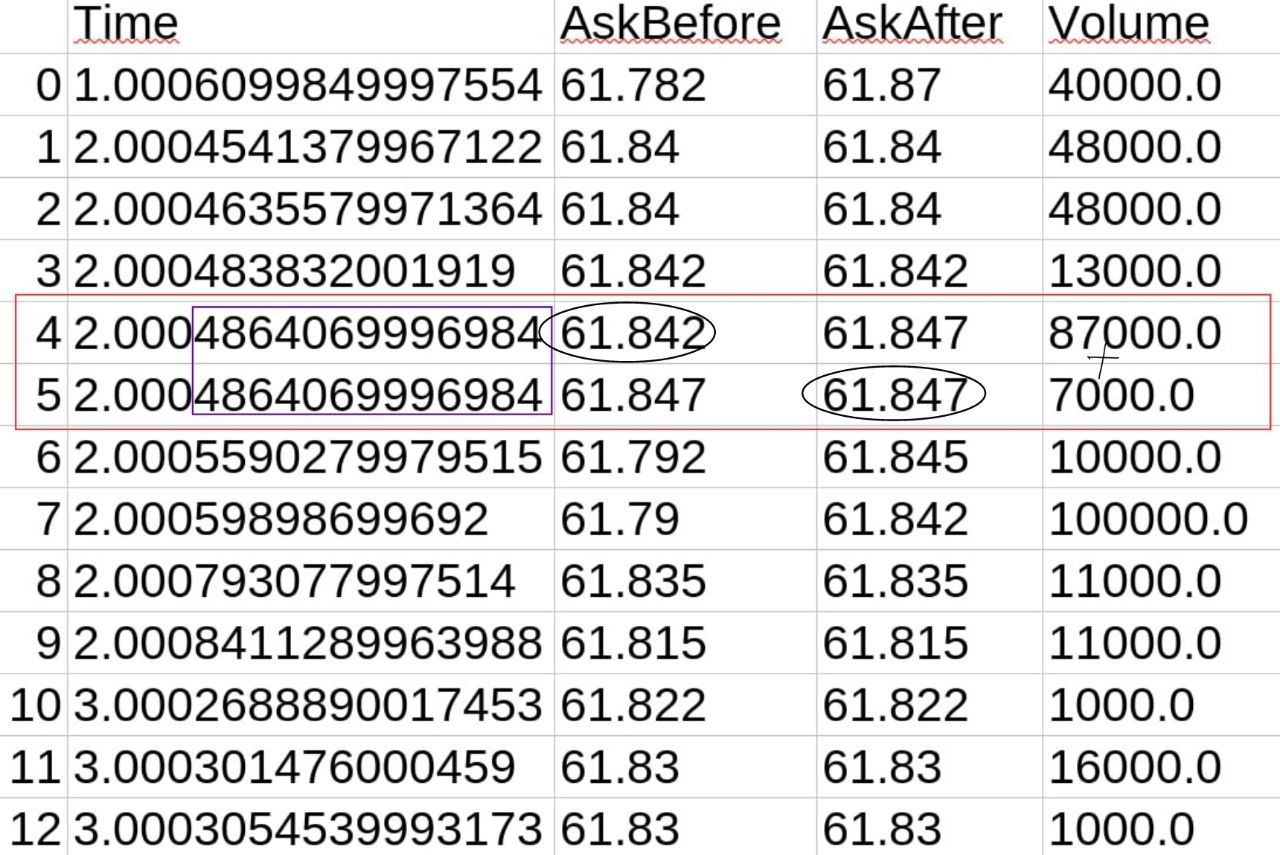
\includegraphics[scale=0.35]{fig/datscsv.jpg}
    \caption{Данные после первого этапа парсинга}
    \label{datacsv}
\end{figure}

\subsection{Выбор инструмента}

Для очень существенной части активов, торгуемых на московской бирже, модель неприменима: в частности,
встречается немало инструментов, по которым совершается порядка нескольких десятков сделок в день (и даже меньше). При этом, почти у всех активовов подавляющее
большинство сделок не поглащает ни одного уровня (те фактическая цена совершения сделки равна аску). В целом, известно, что российский рынок 
характеризуется низким уровнем ликвидности и низким уровнем интенсивности торгов. 
Для подбора параметров и статистических исследовании
нам нужно относительно большое количество данных, к тому же в выводе регрессии мы пользовались малостью промежутков времени, 
поэтому мы остановили выбор на исследовании валютных рынков.
Однако, и среди валютных пар большая часть имеет очень низкую интенсивность торгов, например, CHFRUB\_TOM, CNYRUB\_TOM, HKDRUB\_TOM, 
JPYRUB\_TOM, KZTRUB\_TOM. \par
Для выбора инструмента мы исследовали все, имеющиеся валютные пары и сформировали список наиболее ликвидных (данные за 02.03.2020):

\begin{table}[h!]
    \begin{center}
        \begin{tabular}{|c|c|c|c|c|c|}
            \hline
        Инструмент        & Общее число сделок & Не повлияли на аск & Спайки, среди сдвинувших аск \\ \hline
        USD000UTSTOM      & $41963$ & $95\%$ & $21\%$ \\ \hline
        USD000000TOD      & $13391$ & $86\%$ & $31\%$ \\ \hline
        EUR\_RUB\_\_TOM   & $13383$ & $93\%$ & $32\%$ \\ \hline
        EUR\_RUB\_\_TOD   & $4134 $ & $58\%$ & $42\%$ \\ \hline
        USD000TODTOM      & $1343 $ & $72\%$ & $89\%$ \\ \hline
        EURUSD000TOM      & $915  $ & $91\%$ & $26\%$ \\ \hline
        EUR000TODTOM      & $265  $ & $72\%$ & $89\%$ \\ \hline
        GBPRUB\_TOM       & $234  $ & $64\%$ & $ 0\%$ \\ \hline
        CNYRUB\_TOM       & $167  $ & $51\%$ & $51\%$ \\ \hline
        \end{tabular}
    \end{center}
    \label{tableanalCU}
    \caption{Анализ сделок по наиболее торгуемым валютным парам (03.02.2020).}
\end{table} 

\begin{table}[h!]
    \begin{center}
        \begin{tabular}{|c|c|c|c|c|c|}
            \hline
        Инструмент        & Общее число сделок & Не повлияли на аск & Спайки, среди сдвинувших аск \\ \hline
        USD000UTSTOM & 28361 &    95\% & 69\% \\ \hline
        USD000000TOD & 9624 &     92\% & 61\% \\ \hline
        EUR\_RUB\_\_TOM & 4021 &  79\% & 73\% \\ \hline
        EUR\_RUB\_\_TOD & 2535 &  57\% & 52\% \\ \hline
        USD000TODTOM & 546 &      55\% & 95\% \\ \hline
        EURUSD000TOM & 409 &      93\% & 82\% \\ \hline
        GBPRUB\_TOM & 220 &       60\% & 73\% \\ \hline
        EUR000TODTOM & 168 &      89\% & 100\%  \\ \hline
        \end{tabular}
    \end{center}
    \label{tableanalCU}
    \caption{Анализ сделок по наиболее торгуемым валютным парам (03.03.2021).}
\end{table} 

\begin{table}[h!]
    \begin{center}
        \begin{tabular}{|c|c|c|c|c|c|}
            \hline
        Инструмент   & Общее число сделок & Не повлияли на аск & Спайки, среди сдвинувших аск \\ \hline
        SBER &  $41647$  & $ 96\% $ &  $ 48\% $\\ \hline
        GAZP &  $21566$  & $ 86\% $  & $ 50\% $ \\ \hline
        VTBR &  $17100$  & $ 99\% $ &  $ 34\%$ \\ \hline
        YNDX &  $14110$  & $ 68\% $  & $ 39\% $ \\ \hline
        MGNT &  $10929$  & $ 64\% $  & $ 30\% $ \\ \hline
        LKOH &  $9759 $ &  $ 75\% $ &  $ 35\% $\\ \hline
        ROSN &  $8648 $ &  $ 74\% $ &  $ 39\%$ \\ \hline
        PLZL &  $7121 $ &  $ 56\% $ &  $ 27\% $\\ \hline
        SNGSP & $ 6032$  & $ 60\% $  & $ 24\% $ \\ \hline
        MTLR &  $5985 $ &  $ 46\% $ &  $ 75\%$\\ \hline
        \end{tabular}
    \end{center}
    \label{tableanalSE}
    \caption{Анализ сделок по наиболее торгуемым акциям (03.03.2021).}
\end{table} 

% В паре ликвидных валют EURUSD000TOM происходит лишь порядка пятисот сделок в день. Тем не менее, мы решили исследовать и эту пару,
% поскольу данных (если не слишком сильно их фильтровать) достаточно для обучения модели, в то же время, характер торгов, очевидно,
% другой. \par
% Таким образом, мы решили остановить свой выбор на парах
% USD000UTSTOM и EURUSD000TOM.



\subsection{Аномалии}

Данные характеризуются очень большим числом количеством резких однотиковых скачков аска (см. график \ref{askgraph}). 
В то же время, эти скачки, в целом, не характеризуют
динамику рискового актива, поэтому целесообразно исключить их из исследуемого датасета. \par
Пересечение множеств
сотни самых больших сделок и сотни сделок, сдвинувших аск сильнее всего, пусто. Таким образом, похоже, что ордеров,
которые существенно двигают аск за счёт своего размера на рынке нет, те цена двигается, в основнов, по фундаментальным причинам.
В то же время, эти скачки, в целом, не характеризуют
динамику рискового актива, поэтому целесообразно исключить их из исследуемого датасета.
\begin{figure}
    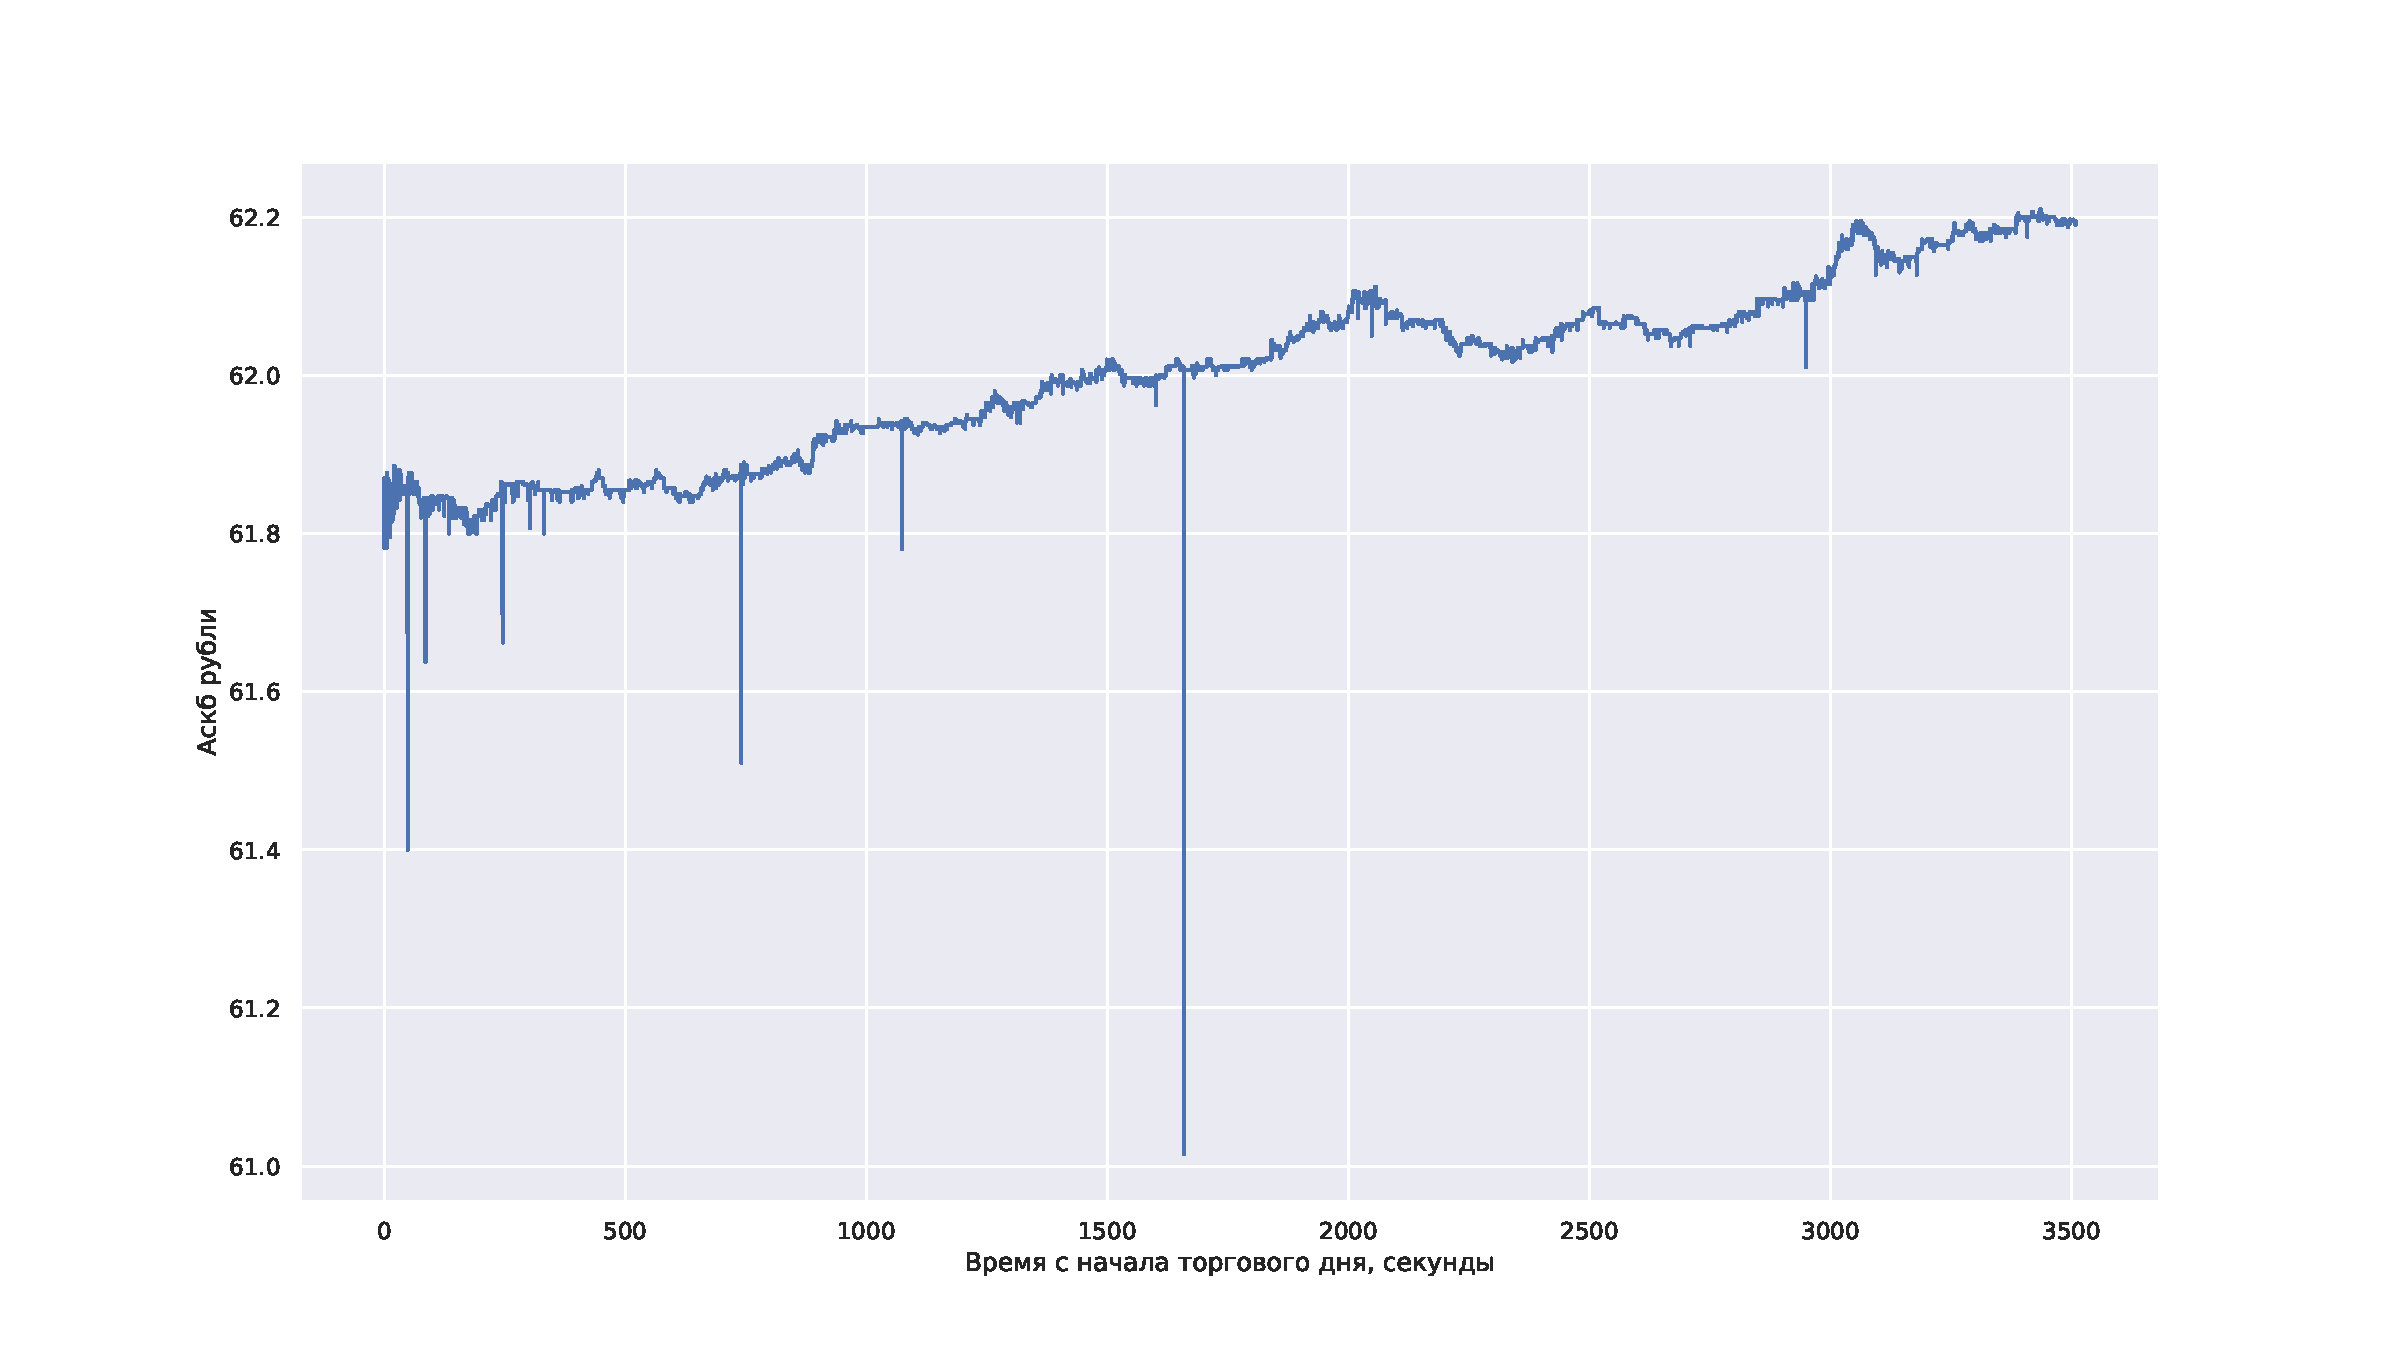
\includegraphics[scale=0.41]{fig/Palki.pdf}
    \caption{График аска USD000UTSTOM в первый час торгового дня}
    \label{askgraph}
\end{figure}


\section{Результаты регрессий на реальных данных}

\begin{table}[h!]
    \begin{center}
        \begin{tabular}{|c|c|c|c|c|c|}
            \hline
        Инструмент        & Общее число сделок & $\rho$ & $\rho ^*$ \\ \hline
        USD000UTSTOM    & $41963$ & $63550^{***}$ & $18345^{***}$ \\ \hline
        USD000000TOD    & $13391$ & $69906^{***}$ & $14649^{***}$ \\ \hline
        EUR\_RUB\_\_TOM & $13383$ & $62892^{***}$ & $2483^{***} $ \\ \hline
        EUR\_RUB\_\_TOD & $4134 $ & $47462^{***}$ & $1675^{**}  $ \\ \hline
        USD000TODTOM    & $1343 $ & $19322^{***}$ & $23534^{***}$ \\ \hline
        EURUSD000TOM    & $915  $ & $9673^{**}  $ & $4417^{*}   $ \\ \hline
        EUR000TODTOM    & $265  $ & $6446       $ & $3750       $ \\ \hline
        GBPRUB\_TOM     & $234  $ & $0.0053     $ & $-0.0132    $ \\ \hline
        CNYRUB\_TOM     & $167  $ & $11214      $ & $1193       $ \\ \hline
        \end{tabular}
    \end{center}
    \label{tableanal}
    \caption{Упругость стакана $\rho$, вычисленная для разных валютных пар.}
\end{table} 

\begin{table}[h!]
    \begin{center}
        \begin{tabular}{|c|c|c|c|c|c|}
            \hline
        Инструмент        & Общее число сделок & $\rho$ & $\rho ^*$ \\ \hline
        SBER &  $41647$  & $ 43257    $ & $ 357819     $ \\ \hline
        GAZP &  $21566$  & $ 31240^{***}    $ & $ 298196^{***}     $ \\ \hline
        VTBR &  $17100$  & $ 2.44e-23 $ & $ 1.49e-23 $  \\ \hline
        YNDX &  $14110$  & $ 24715^{***}    $ & $ 65218^{***}     $ \\ \hline
        MGNT &  $10929$  & $ 19207^{***}    $ & $ 181582^{***}    $  \\ \hline
        LKOH &  $9759 $ &  $307474^{***}    $ & $ 151761^{***}    $  \\ \hline
        ROSN &  $8648 $ &  $65814^{***}     $ & $ 92876^{***}     $ \\ \hline
        PLZL &  $7121 $ &  $11072^{***}     $ & $ 267550^{***}    $  \\ \hline
        SNGSP & $ 6032$  & $ 8652^{***}     $ & $ 137911^{***}    $  \\ \hline
        MTLR &  $5985 $ &  $5031^{***}      $ & $ 59414^{***}     $ \\ \hline
        \end{tabular}
    \end{center}
    \label{tableanal}
    \caption{Упругость стакана $\rho$, вычисленная для разных акций.}
\end{table} 

\subsection{Регрессия USD000UTSTOM}

Как видно из таблицы \ref{usdrubregr}, по порядку и знаку коэффициенты $\lambda$ и $\kappa$ выглядят правдоподобно
(из модели Обижаевой--Ванга следует, что они положительны и много меньше единицы).
В то же время, $\rho$ очень велико по модулю, так что стратегия оптимального исполнения
вырождается в TWAP. 
\begin{figure}
    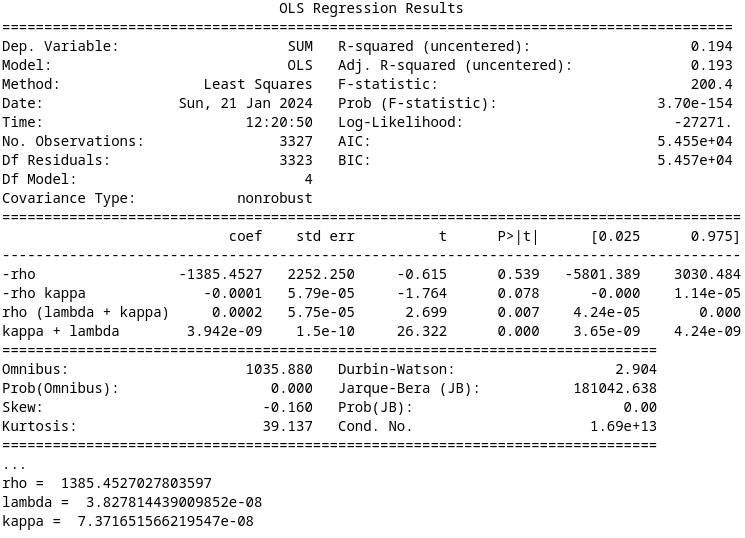
\includegraphics[scale=0.8]{fig/USDRUBregr.png}
    \caption{Регрессия USD000UTSTOM на фильтрованном от скачков датасете}
    \label{usdrubregr}
\end{figure}

\subsection{Регрессия EURUSD000TOM}

Как видно из таблицы \ref{usdeurregr}, по порядку и знаку коэффициенты $\lambda$ и $\kappa$ вновь 
выглядят правдоподобно
(из модели Обижаевой--Ванга следует, что они положительны и много меньше единицы).
В этот раз, $\rho$ довольно мал, так что стратегия оптимального исполнения
отлична от TWAP. Она будет состоять в разделении большей части ордера на две равные доли,
остаток же будет продаваться в промежутке. 

\begin{figure}
    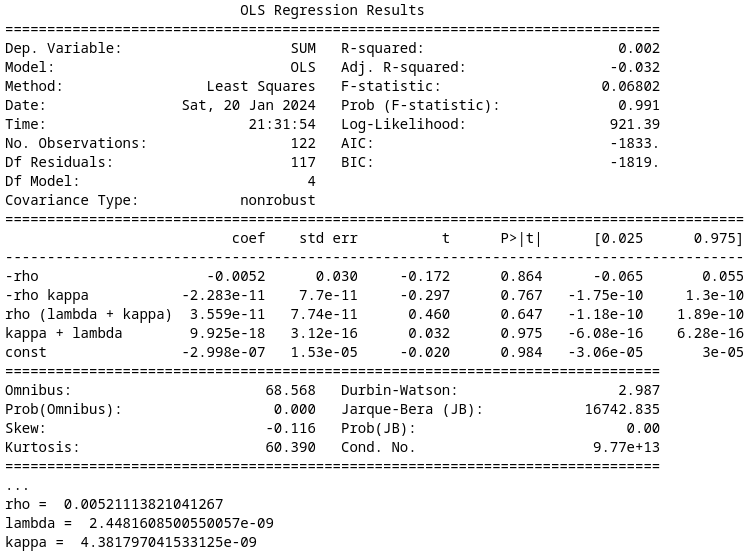
\includegraphics[scale=0.8]{fig/EURUSDregr.png}
    \caption{Регрессия EURUSD000TOM на сыром датасете}
    \label{usdeurregr}
\end{figure}

\subsection{Интерпретация результатов}

Ликвидная пара рубль--доллар оказалась достаточно ликвидной для вырождения стратегии 
в TWAP. Впрочем, мы полагаем, что причина тому не высокая интенсивность торгов и упругость стакана,
но особенность торгов: исчезающе малое количество крупных ордеров. Причем те немногие крупные ордера,
что присутствуют в данных исполняются, в основном, тогда, когда могут поглотить ровно один ценовой уровень.
Таким образом, стакану, в некотором смысле, "не дают повод восстанавливаться": не разрушают его структуру.
\par
Мы считаем, что, вероятнее всего, те же рассуждения верны и для пары евро--доллар. Но выборка небольшая и неотфильтрованная,
аск в ней почти не двигается, этим мы объясняем менее тривиальный результат регрессии. При фильтрации $\rho$ тоже становится большим.
Хотя в этом случае датасет становится настолько малым, что утрачивает даже намёк на репрезентативность.

